\documentclass[14pt]{article}
\usepackage{graphicx}
\usepackage[left=3cm, right=1.5cm, top=1.5cm, bottom=2cm]{geometry}
\usepackage[russian]{babel}
\usepackage[T2A]{fontenc}
\usepackage[utf8]{inputenc}
\usepackage[unicode]{hyperref}
\usepackage{a4wide}
\usepackage{pdfpages}

\begin{document}

\includepdf[pages=-]{title_Ali.pdf}
\clearpage
\tableofcontents
\clearpage
\section{Команда}
\section{Ресурсы}
	\subsection{Сетевой график}
	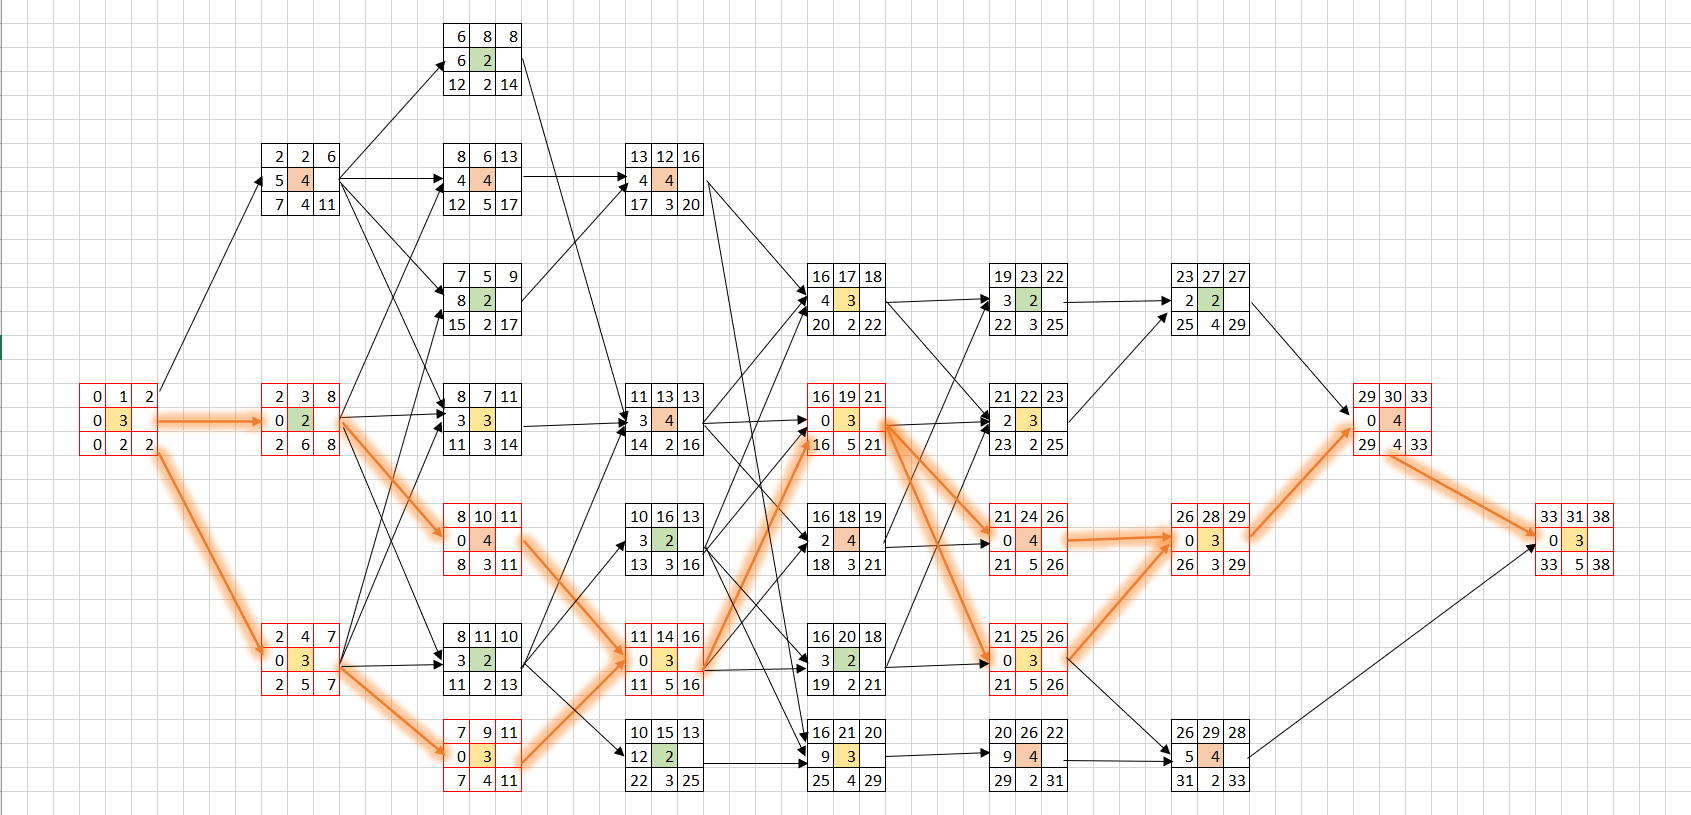
\includegraphics[width=\textwidth]{../img/init_network_graph.png}\\
	В проекте 4 попарно различных кретических пути.
	\subsection{Назначение ресурсов}
	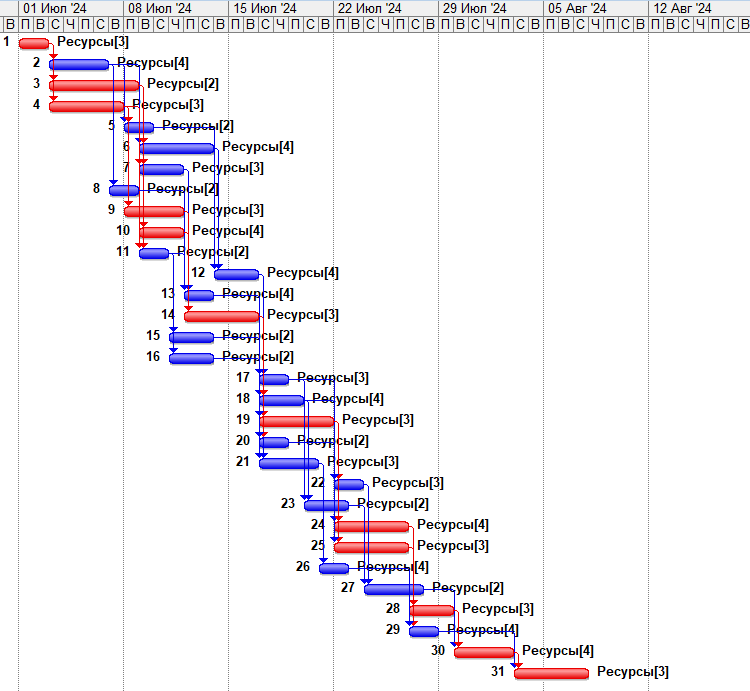
\includegraphics[width=\textwidth]{../img/init_resource_manage.png}
\section{Задача}
	Попробовать уменьшить количество используемых ресурсов до 5 в день,
		меняя при этом длительность работ не более чем на 2 дня и количество ресурсов не более чем на 2 единицы.
	Дату окончания проекта менять нельзя.
\section{Решение}
	\subsection{Первый вариант}
		{\LARGE Что поменяли:}\\
		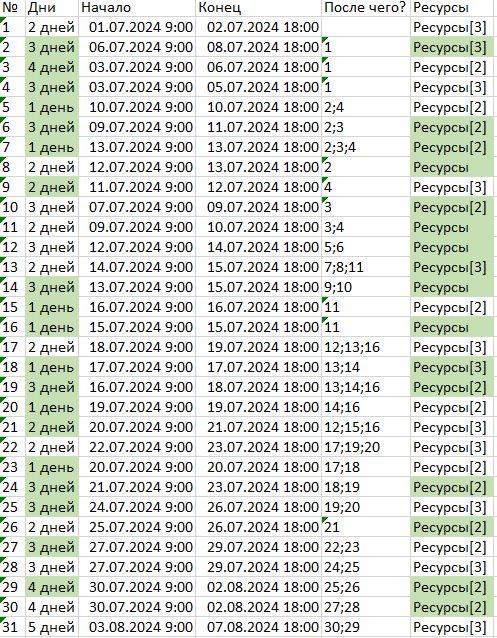
\includegraphics[height=0.6\textheight]{../img/1b1_days_change.png}\\ 
		{\LARGE Как это выглядит:}\\
		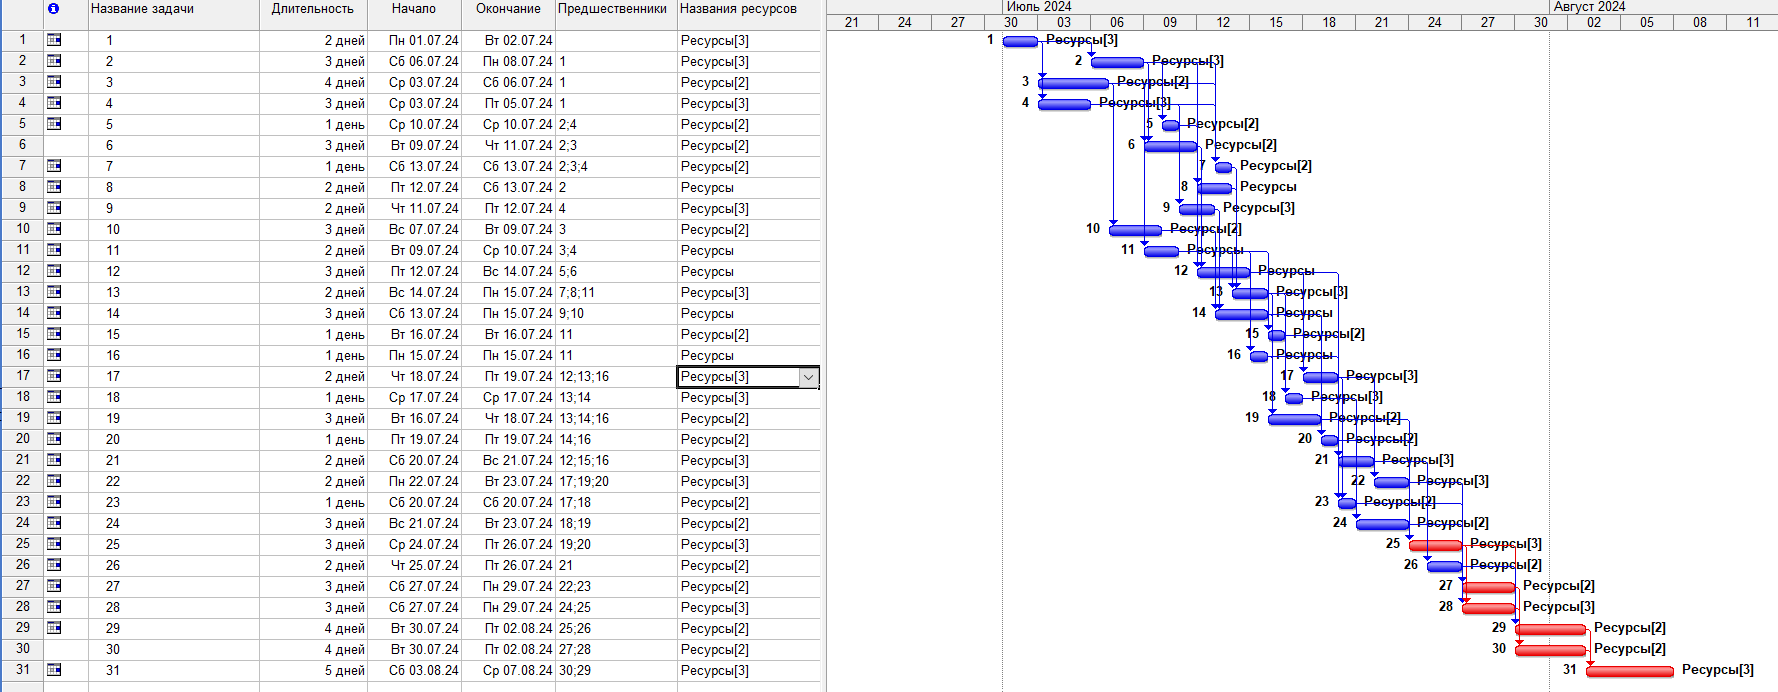
\includegraphics[width=\textwidth]{../img/ot1b1_1.png}\\
		{\LARGE Cколько оно тратит:}\\
		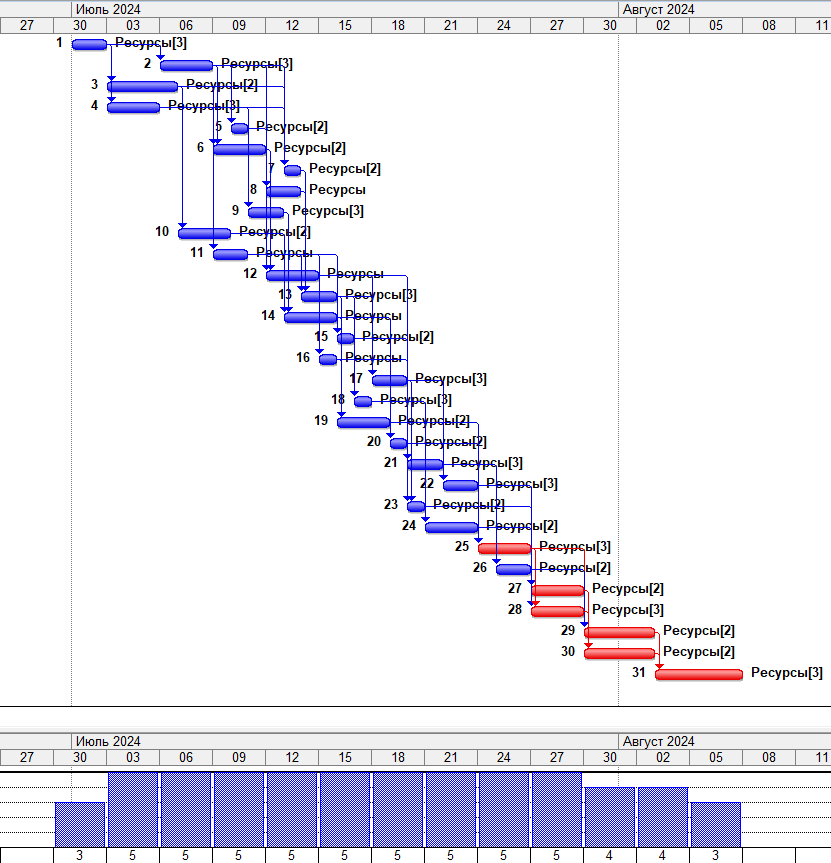
\includegraphics[width=\textwidth]{../img/1b1_answer.png}\\ 
	\subsection{Второй вариант}
		Попробуем найти другое решение, чтобы количество изменений было поменьше.
		Конечно, невозможно просто уменьшить число правок.
		Для этого потребуется место, которое можно получить из задач, уменьшенных на 1 день.
		
		Мы сократили количество изменений с 27-ми до 25-ти.
		Дальнейшее улучшение даже если воможно, то крайне затруднительно.\\
		{\LARGE Что поменяли:}\\
		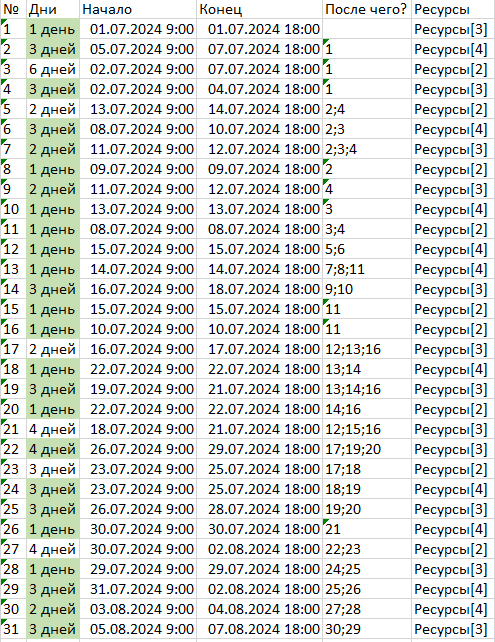
\includegraphics[height=0.6\textheight]{../img/1a2_days_change.png}\\ 
		Внешне кажется, что ничего не поменялось, но изменения есть.
		Их можно заметить, к примеру, посмотрев на задачи 6 и 11.\\
		{\LARGE Как это выглядит и сколько оно тратит:}\\
		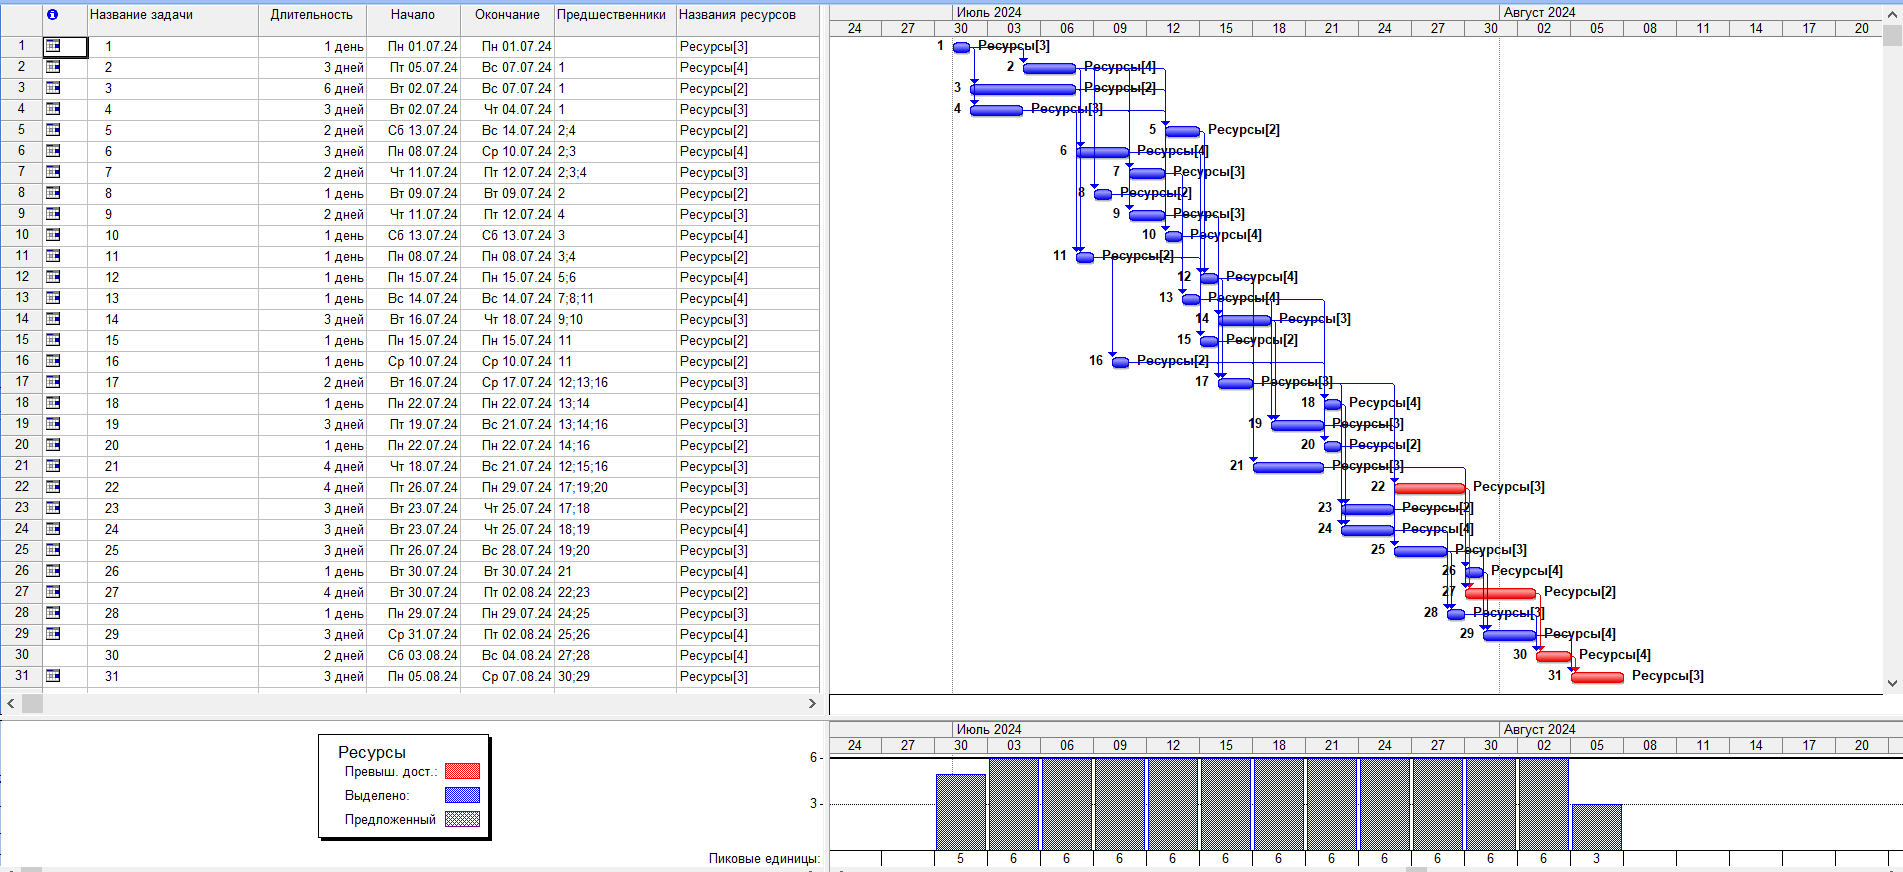
\includegraphics[width=\textwidth]{../img/1a2_answer.png}\\ 
	\subsection{Третий вариант}
		Покажем ещё какое-нибудь решение:
		{\LARGE Что поменяли:}\\
		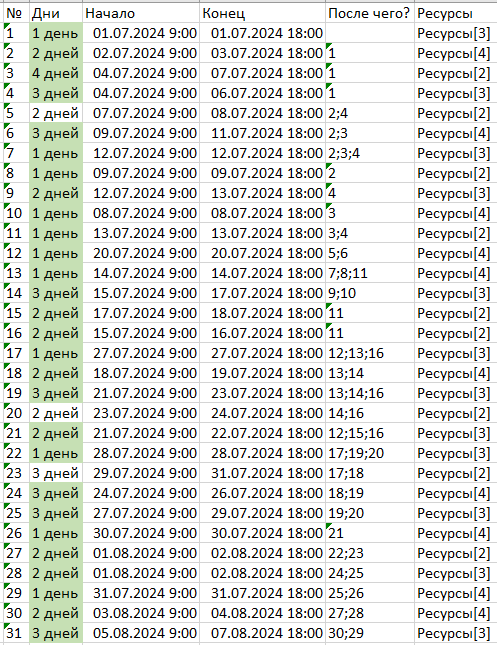
\includegraphics[height=0.6\textheight]{../img/1a3_days_change.png}\\ 
		{\LARGE Как это выглядит и сколько оно тратит:}\\
		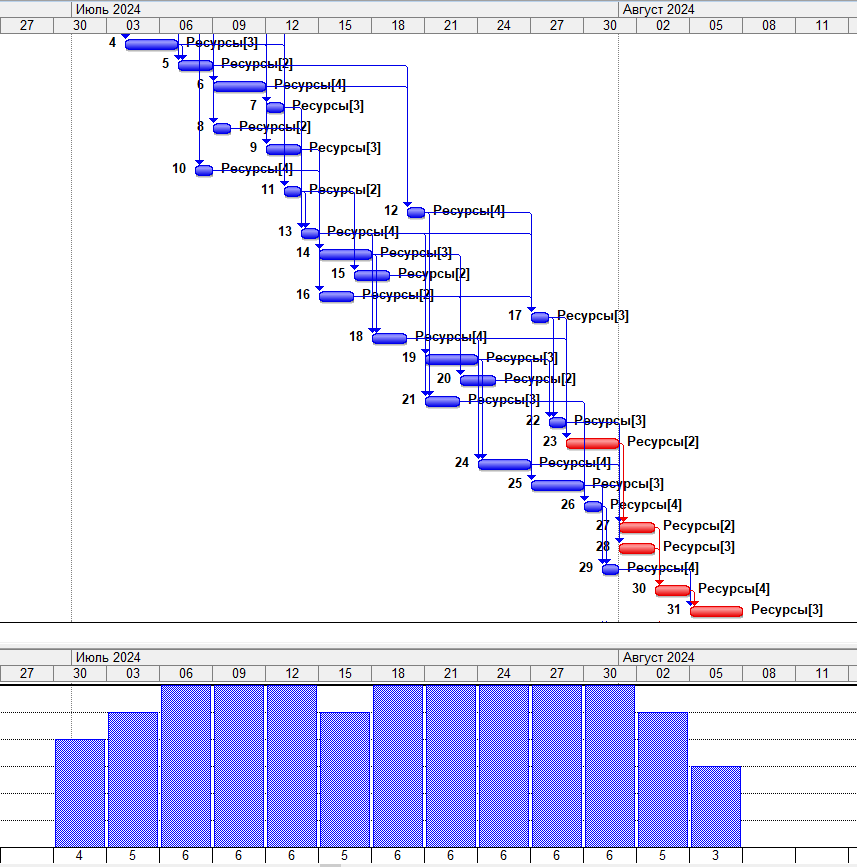
\includegraphics[width=\textwidth]{../img/1a3_answer.png}\\ 
\end{document}
